\chapter{Improvement of the rejection of the internal Thallium-$208$ background}
\label{ch:timediff}

At the end of September $2018$, the $34$ enriched-Selenium source foils were installed on the demonstrator.
At this time, the internal \Tl\ and \Bi\ activities had already been measured by the BiPo detector, as well as the \Rn\ concentration inside the tracker chamber.
The \Rn\ targeted level is reached, and an upper limit have been provided for the internal \Bi.
However, the activity of \Tl\ was revealed higher than expected.

We described in the previous chapter the impact of these activities on the final detector sensitivity to the $\zeronu$ decay, and optimised topological selections allowed to improve it.
In the current chapter, we focus on rejection techniques peculiarly adapted to reject internal \Tl\ events, while selecting a significant proportion of $\zeronu$ signal.


\section{Motivations}

In Chapters~\ref{ch:detector} and \ref{ch:sensitivity}, we presented the specifications set on the background activities, in order to reach an unprecedented limit on the $\zeronu$ process half-life in $5$ years, with $100$~kg of the \Se\ isotope, with the final SuperNEMO detector.
Tab.~\ref{tab:real_target_act} summarise the target \Tl, \Bi\ and \Rn\ activities, and give a comparison with those measured by the collaboration.
We achieve the specified level of \Rn\ isotope inside with an air flow rate of $2$~m$^{3}$/h inside the wire chamber.
The BiPo detector was only capable of giving an upper limit on the \Bi\ level of $\mathcal{A}^{\text{Bi}}~<~290~\mu$Bq/kg, and future precise measurements with SuperNEMO demonstrator will constraint this value.
The BiPo measurements also showed that the \Tl\ contamination is about $30$ times greater than expected.
This level of activity has no implications for the demonstrator, as only one \Tl\ event is expected in the [$2.7$;$3.15$]~MeV energy region, after cut-off optimisations, with a $17.5$~kg.y exposure.
On the other hand, this background could be harmful for the final detector, with $21$ \Tl\ events expected in the region of interest [$2.6$,$2.95$]~MeV, for a $500$~kg.y exposure.
To overcome this effect, it is interesting to set a specific method designed to reject \Tl\ events.

In the next section, we describe the specific features of the Thallium internal background.
We develop a new technique of rejection, especially designed to identify internal \Tl\ events, based on electron Time-Of-Flight computation.

\section{The internal \Tl\ background}

Trace quantities of naturally-occurring radioactive isotopes inside the source foils can occasionally produce two-electron events, and thus can mimic $\beta\beta$-decay events.
The \Tl, a progeny of \Th, is one of the largest contribution to the internal background.
In fact, as explained in Chapter~\ref{ch:detector}, two electrons can be produced via $\beta$-decay followed by a M\o{}ller scattering, $\beta$-decay to an excited state with the subsequent internal conversion, or due to Compton scattering of the de-excitation photon (Fig.~\ref{fig:internal_contamination}).
%% The ultimate internal background for $\zeronu$ experiments is the $\twonu$ decay of the studied isotope.
%% When present in the source foils, \Tl\ and \Bi\ can mimic the $\zeronu$ signal by different processes (see Fig.~\ref{fig:internal_contamination}).

All the possible transitions for the \Tl\ isotope are presented in Fig.~\ref{fig:Tl_scheme}.
\begin{figure}
  \centering
  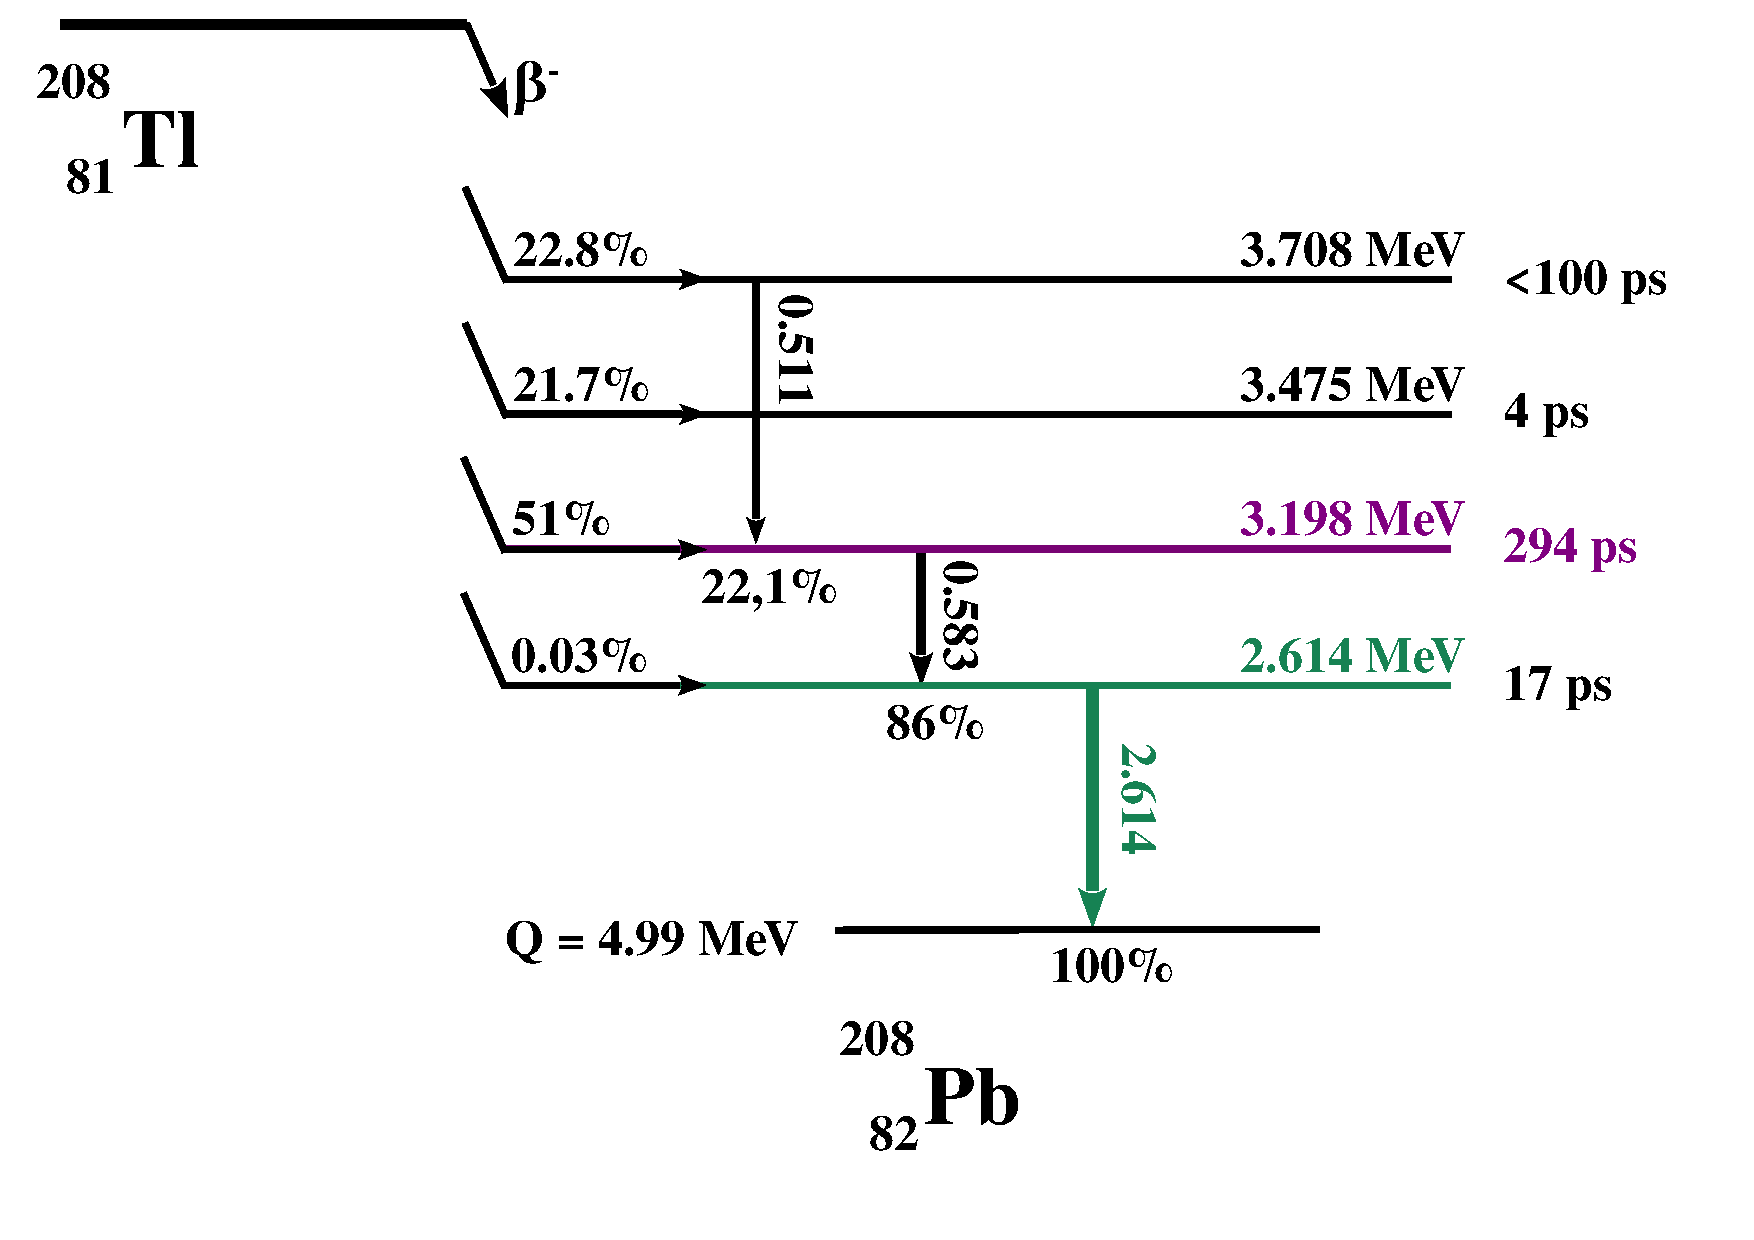
\includegraphics[width=13cm]{timedifference/fig_timediff/Tl_decay_scheme.pdf}
  \caption{A simplified disintegration scheme for the \Tl\ isotope.
    $81$~\% of the disintegration pass through the $294$~ps metastable energy level (orange).
    All disintegration go through the $2.615$~MeV energy level (green), where an orbital electron is ejected in $0.246$~\% of the cases through the internal conversion process.
  \label{fig:Tl_scheme}}
\end{figure}
This shows that \Tl\ always $\beta$-decays to an excited state of the \Pb\ daughter nuclei.
In more than $99$~\% of the decays, at least 2 $\gamma$'s are expected after the $\beta$ emission.
For $\zeronu$ detection, the most dangerous mode of $\beta\beta$-like events production comes from the internal conversion of the $2.615$ MeV-$\gamma$, resulting in two electrons emitted with a high energy sum.

\subsection{The internal conversion process}

An excited nucleus will practically constantly achieve a transition to a lower state by one of two processes: the emission of a $\gamma$-ray, or the ejection of one of the orbital electrons.
The latter, called \emph{internal conversion} (frequently abbreviated IC), is a second-order process, where one electron couples to one of the nucleon inside the excited nucleus.
After bringing the energy of the nuclear transition, the electron is ejected from the atom.
Thus, in such a radioactive decay, the de-excitation energy of the nucleus is transferred \emph{directly} to a $j$-shell electron ($j=K,L,M...$).
The high-energy electron is therefore emitted not from the nucleus, but from the atom, and carry off the energy
\begin{equation}
E_{IC} = E_{\gamma}-E_{j}\qquad (j=K,L,M...)\,,
\end{equation}
where $E_{j}$ is the binding energy of the electron in the $j$-shell, and $E_{\gamma}$ is the energy of the $\gamma$-ray.

This mechanism is possible because there is a non-zero probability of finding the electron within the nucleus, that is to say, the wave-function of the electron can penetrate the volume of the nucleus.
Consequently, due to their high nuclear penetration, electrons coming from the $1s$ state are more likely to be ejected (this transition is called $K$ internal conversion).
Although electrons coming from $2s$, $3s$ and $4s$ states ($L$, $M$ or $N$ internal conversions) have also a non-zero probability to undergo this process.
After the electron ejection, the hole in the corresponding shell is filled by an electron from a higher energy level, emitting characteristic $X$-rays, Auger electrons, or both.

For a given transition, the internal conversion coefficient of the electron in the $j$-shell, is defined by
\begin{equation}
\alpha_{j}=\frac{P_{IC, j}}{P_{\gamma}}\,,
\end{equation}
%% \begin{equation}
%% \alpha_{K}=\frac{P_{IC, K}}{P_{\gamma}}\,,
%% \end{equation}
where $P_{IC,j}$ is the $j$ conversion electron emission probability, and $P_{\gamma}$ is the $\gamma$-ray emission probability.
The total coefficient is
\begin{equation}
  \alpha_{T}=\sum_{j=K,L,M\cdots}\alpha_{j}\,.
\end{equation}
These coefficients are given in Tab.~\ref{tab:IC_prob}, for the $2.615$~MeV energy level of the \Tl\ decay scheme.
\begin{table}[h]
  \centering
  \begin{tabular}{|c|c|c|c|c|}
    \hline
    Emission probability (\%) & $\alpha_{K}$ (\%) & $\alpha_{L}$ (\%) & $\alpha_{M}$ (\%) & $\alpha_{T}$ (\%) \\
    \hline\hline
    $100$ & $0.1708$ &    $0.0292$ &  $0.00685$  &    $0.246$ \\
    \hline
  \end{tabular}
  \caption{Internal conversion coefficients for the $2.615$~MeV $\gamma$-ray of the \Tl\ decay scheme.
    \label{tab:IC_prob}}
\end{table}
Therefore, in $0.246$~\% of the cases, the \Pb\ excited nucleus will undergone an internal conversion corresponding to the $2.615$~MeV energy level.


\subsection{Selection of \Tl\ disintegrations in the 2e channel}

The \Tl\ can present a $2e$ electrons topology, when after the $\beta$ emission, an electron is ejected from the atom through internal conversion.
Especially, when this energy transfer corresponds to the $2.615$~MeV $\gamma$-ray, the ejected electron carry off a significant energy, depending on its initial binding energy with the nucleus.
An orbital electron from the $K$-shell is ejected with an energy $E_{IC,K}=2.526$~MeV, for instance.
In such a case, the \Tl\ disintegration can be identified in the $2e$ topology.
As one of the two electrons measured with a high energy, this decay is likely to contribute to the background of the $\zeronu$ of \Se, or even \Nd.
In Fig.~\ref{fig:Emin_Emax_Tl} is presented the individual energy spectra for $2e$ topologies for \Tl\ simulations inside the source foils.
\begin{figure}
  \centering
  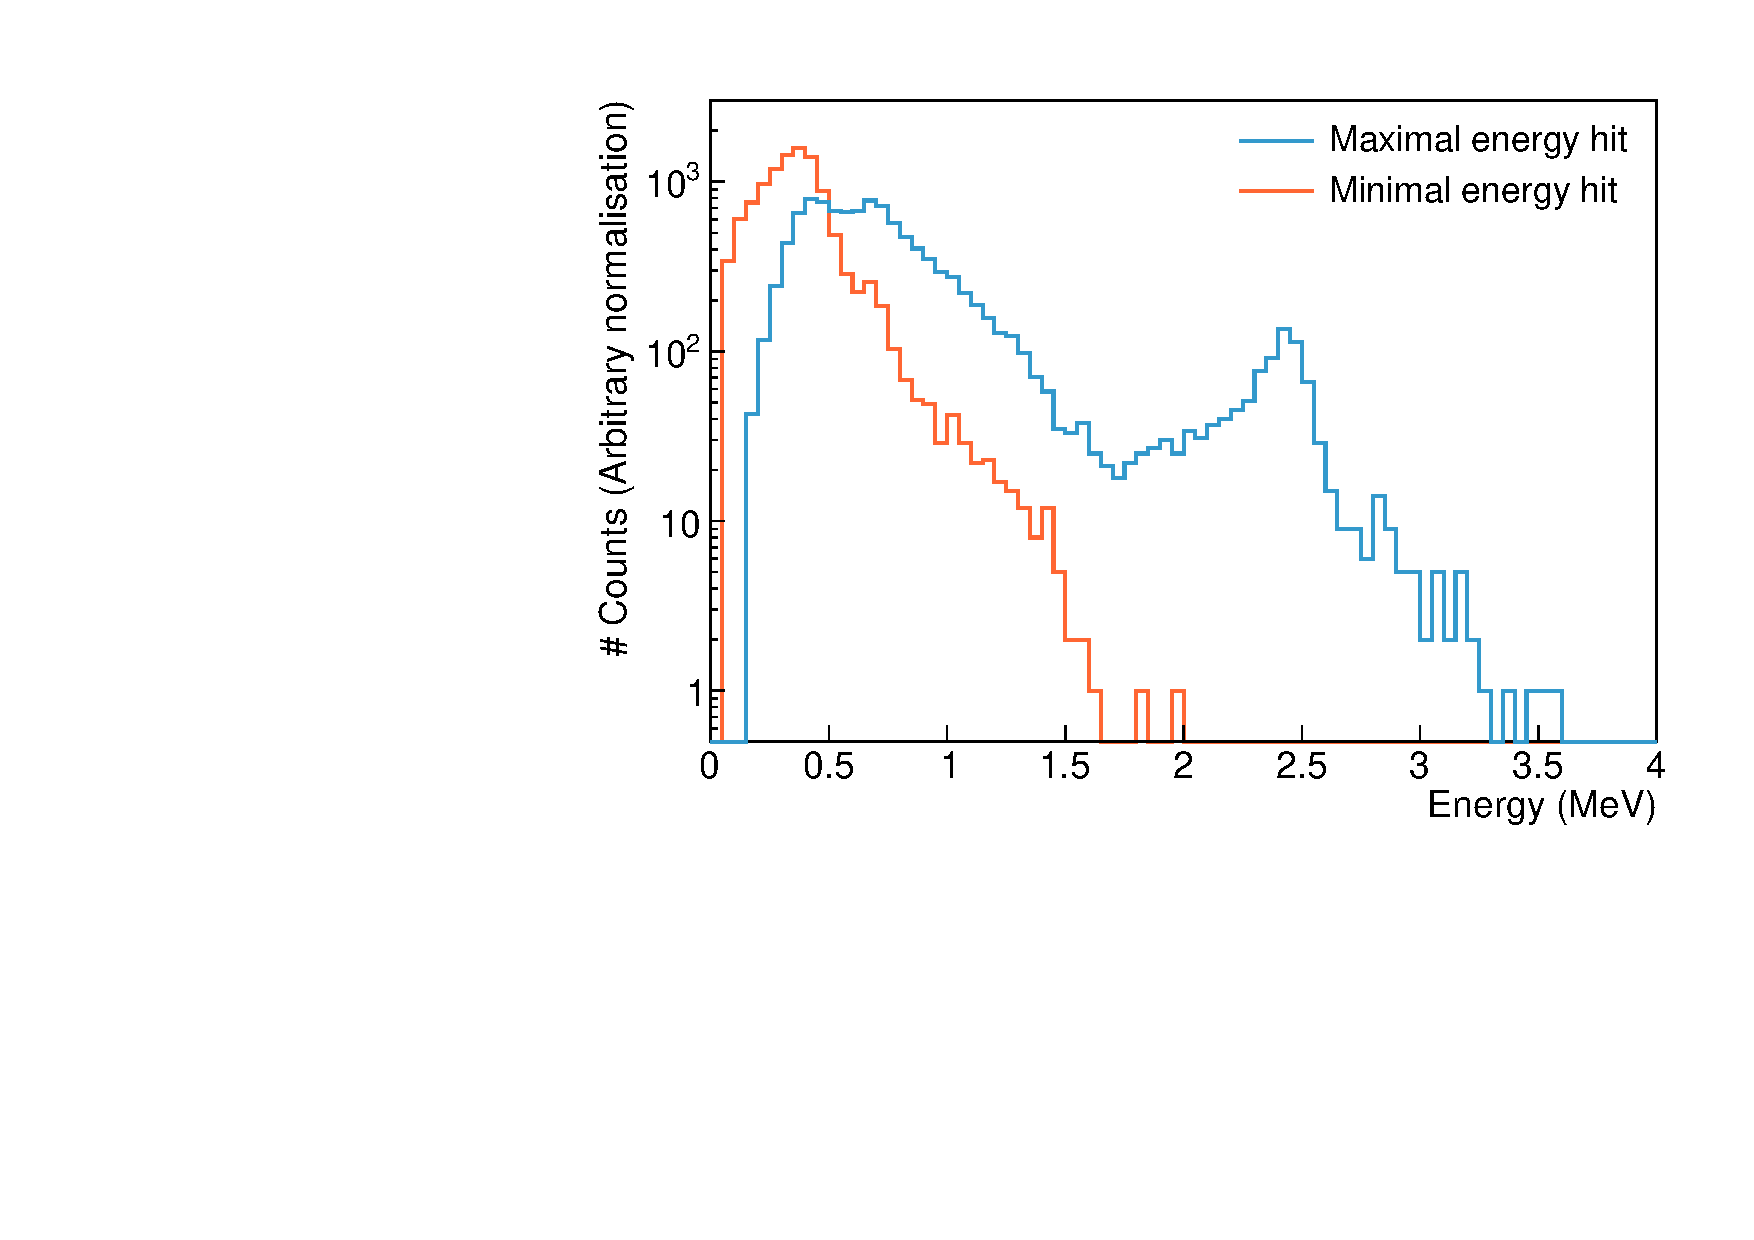
\includegraphics[width=13cm]{timedifference/fig_timediff/energy_spect_min_max_208Tl.pdf}
  \caption{Individual energy spectra for selected $2e$ topologies of \Tl\ decays simulated inside the source foils.
    Calorimeter hit of minimal energy (red) and maximal energy (blue).
    Spectra are arbitrarily normalised.
    The [$2.7$;$3.2$] ROI is represented by grey dashed lines.
    \label{fig:Emin_Emax_Tl}}
\end{figure}
An usual technique to reject \Tl\ background consists in distinguishing $2e$ topologies for which one of the two calorimeter hits have an energy greater than $2.7$~MeV.
The energy resolution of the demonstrator being improved compared with the one of NEMO-$3$, this selection is efficient.
This cut-off allow to reject $0.61$~\% of the \Tl\ internal events, while rejecting only $0.11$~\% of $\zeronu$ events.

In the $2e$ channel, optimised topological cut-offs, based on time-of-flight computation and the distance between vertices, were presented in the previous chapter.
They are mostly efficient in rejecting the non-internal \Rn\ events.
In the next section, we remind and precise the internal probability computation, and present a new selection, also based on the time-of-flight computation, to reject the \Tl\ background.

\section{Rejection of \Tl\ with a time-of-flight criterion}

\begin{itemize}
\item Un des deux gamma est retardé de 294 ps, puis conversion interne -> donner le proportion (nb d'ev attendus, dans la ROI). proportion déjà donnée, je pense que tu veux dire le nombre d'événements attendus pour une contamination fixée.
\item Avant d'entrer dans le détail préciser le principe de la réjection par temps de vol.
  L'électron de plus haute énergie est en retard, avec un retard en moyenne de 294 ps pour la plupart des niveaux (discuter un peu le schéma de désintégration, dans quel cas il sera en retard).
  Ensuite dire que tu as quantifié le pourcentage d'électrons de haute énergie en retard avec une simulation "parfaite" i.e. avec une résolution en  temps  nulle.
  A comparer avec le chiffre donné précédemment (issu d'une étude du schéma de désintégration.)
\end{itemize}

%% Internal conversion occurs after $\beta$ or $\alpha$ radioactive decays leaving the nucleus excited.
%% Then a $\gamma$ particle is emitted and transfers its energy to an atomic electron which results in ejection of this electron from the atom.
%% The emitted electron has an energy corresponding to the energy of previously excited nucleus reduced by the electron binding energy.
%% After the internal conversion, electrons reorganise.
%% The hole in internal layer is filled by an electron from an external layer (emitting an X ray).\\
%% The probability for an atomic electron to be ejected decreases with the initial binding energy.
%% Thus, electrons from K layers have a higher probability to be converted (see Fig.~\ref{fig:Tl_IC}).

\subsection{The internal probability}

This tool, which aims to reject non-simultaneous events, is presented in detail in Chapter~\ref{ch:detector}.
As part of the analysis pipeline, it is widely employed in NEMO-$3$ and SuperNEMO, for background rejection purposes.
We examine an example of its usefulness in Chapter~\ref{ch:sensitivity}.
Nevertheless, for reasons to be given latter, in the current chapter, we need to perform our own calculation of internal probability, after the reconstruction pipeline.
This is, therefore, an opportunity to come back to this tool and to clarify certain points.
The calculation of the internal $\chi^{2}$ is reminded in Eq.~\eqref{eq:int_chi2_electrons}, for two detected electrons, as a function of the expected times, $t^{\text{exp}}$, the experimentally measured times, $t^{\text{meas}}$, as well as the total uncertainty on the time measurement:
\begin{equation}
  \chi^{2}_{int}=\frac{((t^{\text{meas}}_{1} - t^{\text{exp}}_{1}) - (t^{\text{meas}}_{2} - t^{\text{exp}}_{2}))^{2}}{\sigma_{t_{1}}^{2}+\sigma_{t_{2}}^{2}+\sigma_{\beta_{2}}^{2}+\sigma_{\beta_{1}}^{2}+\sigma_{l_{1}}^{2}+\sigma_{l_{2}}^{2}}\,.
  \label{eq:int_chi2_electrons}
\end{equation}
The compenents of the total time uncertainty are bring by the calorimeter performance ($\sigma_{t_{i}}$), the uncertainty on particle energies ($\sigma_{\beta_{i}}$) and the uncertainty on track lengths ($\sigma_{l_{i}}$).
%%chap detecteur changer sigmas et t^th
%%ce chap vérifier notation steven sigma l
In the official SuperNEMO reconstruction pipeline, ${\sigma_{l}=\sigma_{l_{1}}=\sigma_{l_{2}}=0.07}$~ns for electrons.
As, therein chapter, we are predominantly focusing on the $2e$ channel to reject the \Tl\ background, we would optimise this parameter to describe accurately the internal events.

One way to examine if $\sigma_{l}$ is well-evaluated is to look at the flatness of the internal probability distribution for $\zeronu$ events in the $2e$ topology, for which a flat distribution is expected.
Indeed, the slope of this distribution provides pertinent information to check the estimation of uncertainties.
The flatter the distribution, the more correctly uncertainties are estimated.
We perform a lineal fit of the \Pint\ distribution on $]0.1;1]$, to avoid the peak at low internal probabilities, and we define the \emph{flatness parameter} $a_{F}$ as the slope of this fit.
The optimisation then consists in finding the value of $\sigma_{l}$ for which the parameter $a_{F}$ is cancelled.
We compute the \Pint\ distribution for simulations of $\zeronu$ decays inside the source foils.
We select merely $2e$ topologies by using the first order cuts, presented in Chapter~\ref{ch:sensitivity}, such that the internal hypothesis is almost certain to be verified.
In Fig.~\ref{fig:flatness} is given the slope $a_{F}$ as a function of $\sigma_{l}$.
\begin{figure}
  \centering
  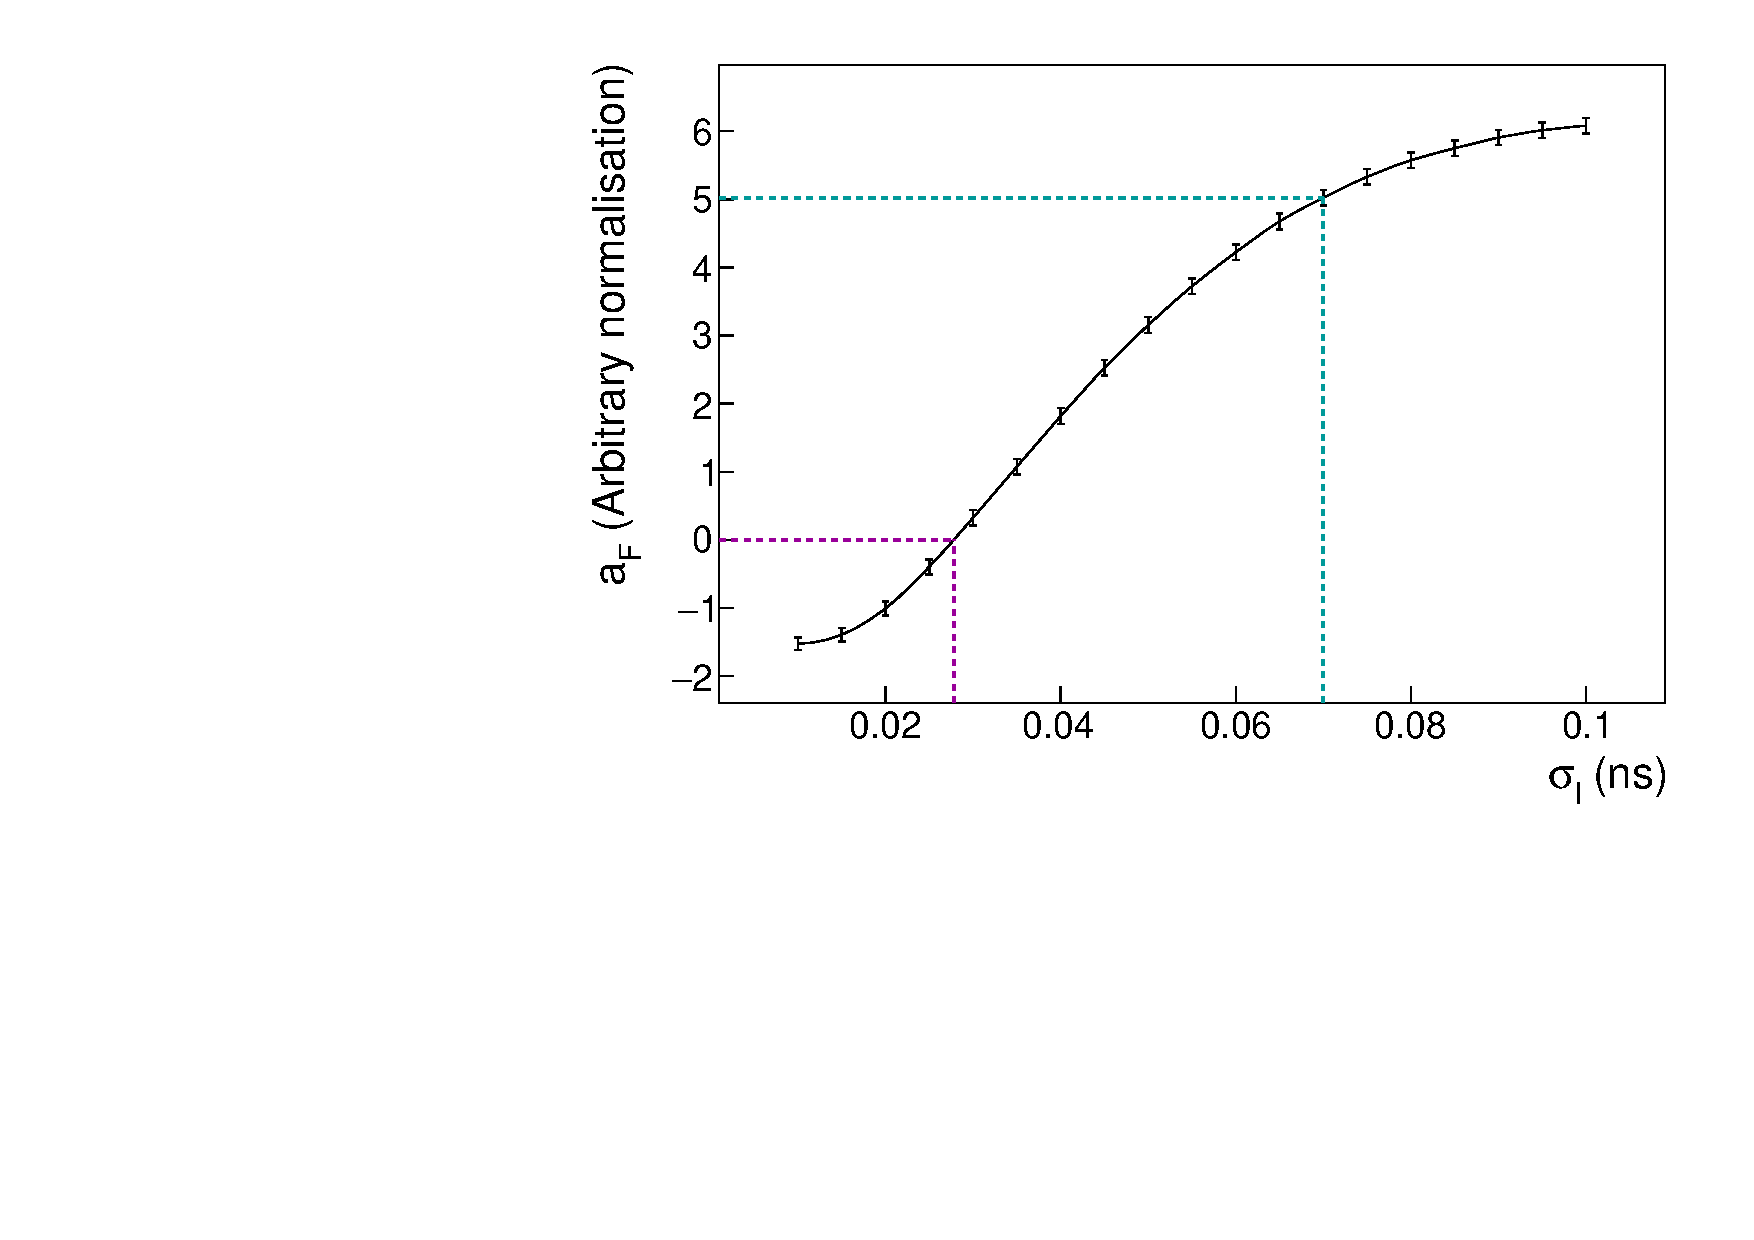
\includegraphics[width=13cm]{timedifference/fig_timediff/flatness.pdf}
  \caption{Slope $a_{F}$ as a function of the time uncertainty due to the reconstructed track length $\sigma_{l}$.
    The former value used in the SuperNEMO reconstruction pipeline is pointed out by blue dashed lines.
    The value kept for $\sigma_{l}$ is the one for which $a_{F}=0$, $\sigma_{l}~=~0.0278~\pm~0.0008$~ns, showed by purple dashed lines.
    The errors made on the $a_{F}$ fit parameter are represented by the grey filled area.
    \Pint\ is calculated for $\zeronu$ decays simulated inside the source foil, with first order cut-offs applied.
    \label{fig:flatness}}
\end{figure}
For $\sigma_{l}=0.07$~ns, $a_{F}>0$, revealing an overestimation of uncertainties in the computation of the internal $\chi^{2}$.
The optimised value, kept for the further analysis, is $\sigma_{l}~=~0.0278~\pm~0.0008$~ns.
In Fig.~\ref{fig:Pint_comparison} is displayed the internal probability distributions for two values of the $\sigma_{l}$ parameter: for the former value $\sigma_{l}=0.07$~ns and for the optimised value $\sigma_{l}=0.0278$~ns.
\begin{figure}
  \centering
  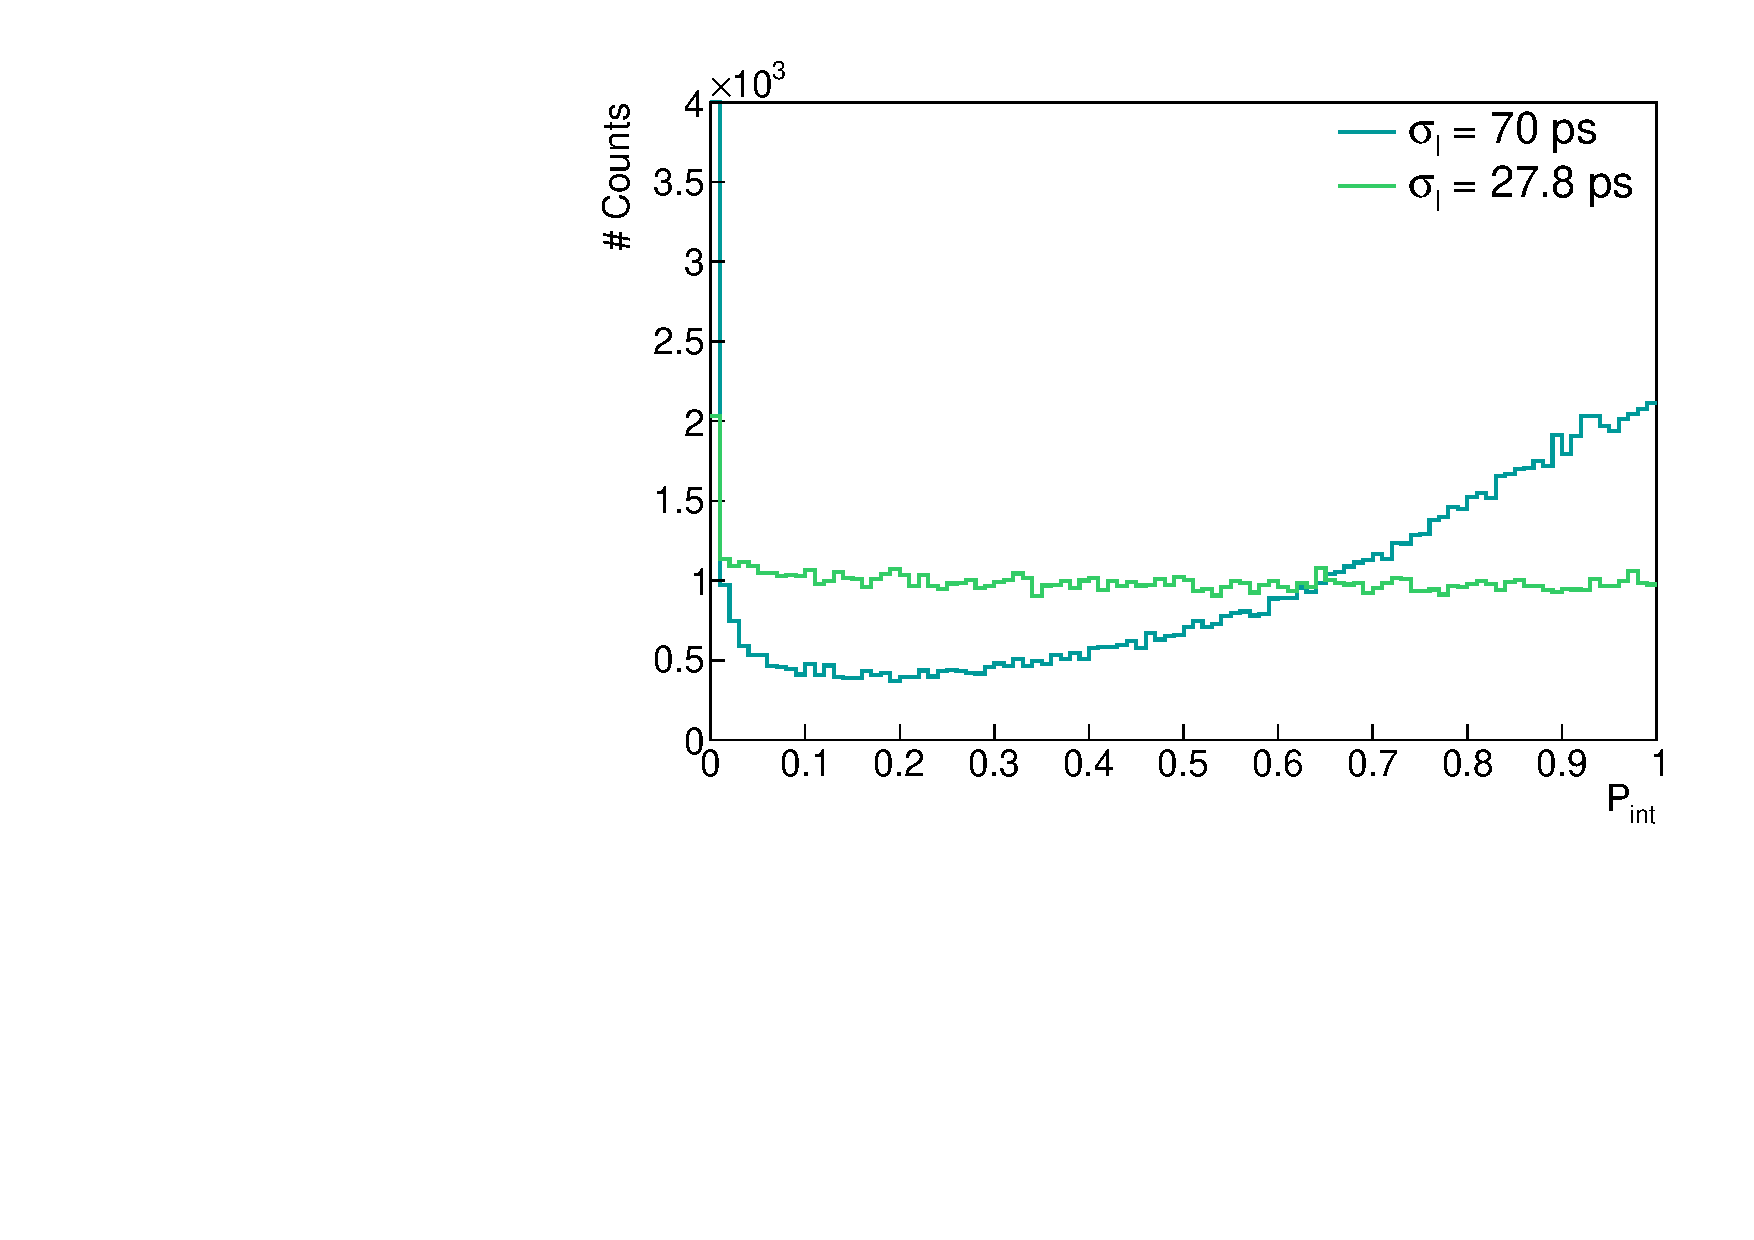
\includegraphics[width=13cm]{timedifference/fig_timediff/Pint_comparison.pdf}
  \caption{Internal probability distributions for $\sigma_{l}=0.07$~ns (blue) and $\sigma_{l}=0.0278$~ns (green).
    \Pint\ is calculated for $\zeronu$ decays simulated inside the source foil, with first order cut-offs applied.
    \label{fig:Pint_comparison}}
\end{figure}
A more complete analysis would compare the simulated track lengths with the reconstructed ones, for different energy sets of mono-kinetic electrons.
Nevertheless, our optimisation is good enough for the current analysis.
We use this optimisation for the rest of this analysis, and discussion is in progress to modify this parameter in the SuperNEMO software.

The internal probability is principally designed to reject non-simultaneous events coming from the source foil.
Therefore, it is extremely effective in rejecting \Rn\ events produced far from the source foils.
The internal probability is however not suited for \Tl\ disintegrations occurring within the foils, because of the metastable state could delay significantly the electron with higher energy.
So we would set up a new law of probability that would express the hypothesis that a given event is an internal \Tl\ event.

\subsection{The exponential probability for \Tl\ events}

According to the disintegration scheme of the \Tl\ isotope (Fig.~\ref{fig:Tl_scheme}), there is an $81~\%$ probability of passing through the $294~$ps metastable level.
After that, to attain the ground state of \Pb, the excited nucleus has $100\%$ of probability to decay through the $2.615$ MeV energy level.
At this occasion, in $0.246\%$ of cases (Tab.~\ref{tab:IC_prob}), one of the orbital electrons is ejected from the atom following the internal conversion process.
To summarise, for $0.16$~\% of the total \Tl\ decays, a $\beta$ particle is emitted, and a delayed orbital electron is ejected through internal conversion of the $2.6$ MeV-$\gamma$.
We aim to use this delayed electron to discriminate \Tl\ internal background from the $\zeronu$ signal.

\subsubsection{Exponentially modified Gaussian}

For a given \Tl\ disintegration, we define the $\Delta t$ parameter as the difference of arrival time between the firstly emitted $\beta$ particle and the delayed IC electron.
Supposing SuperNEMO would perfectly measure the particles' times and energies, the $\Delta t$ probability density function would be an exponential, with the decay parameter $\tau=294$~ps.
We introduced in Chapter~\ref{ch:detector} the internal probability analysis tool.
At this occasion, let us described the components entering in the computation of the total uncertainty on time measurement for the SuperNEMO calorimeter.
To take into account measurement uncertainties, we define a Gaussian distribution centred around $\mu=0$, with a width set up by the $\sigma=\sigma_{tot}$ parameter, detailed in Eq.~\eqref{eq:sigma_tot}.
Therefore, to properly describe the $\beta$+IC delayed \Tl\ events, we have to convolve the exponential and the Gaussian distributions.

\subsubsection{Probability density function}

In Fig.~\ref{fig:Pexp} we show $E \otimes G(\tau,\mu,\sigma)$, the convolution of an exponential function and a Gaussian function.
\begin{figure}
  \centering
  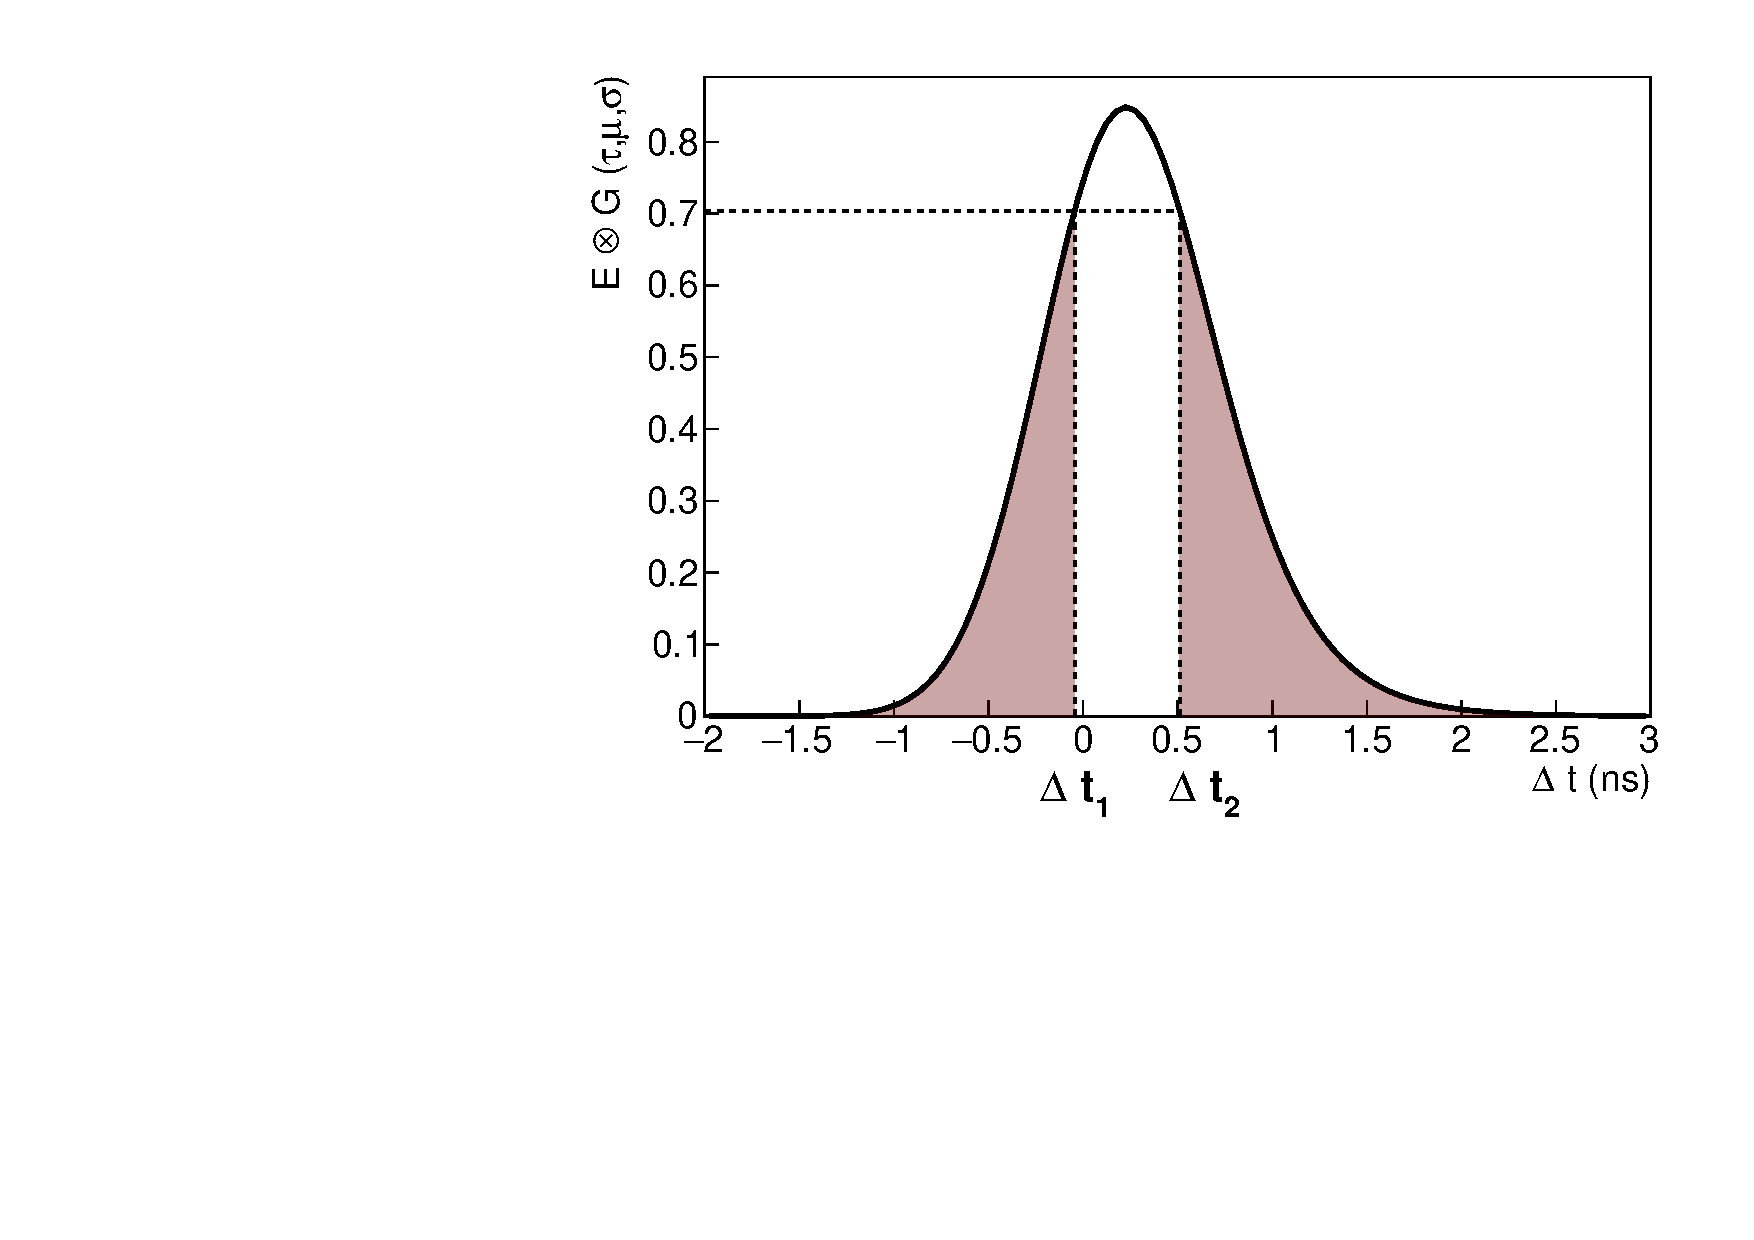
\includegraphics[width=13cm]{timedifference/fig_timediff/proba_expo.pdf}
  \caption{Normalised convolution distribution $E \otimes G (\tau,\mu,\sigma)$.
    The parameters are $\tau=0.294$~ns, $\mu=0$~ns and $\sigma=\sigma_{tot}$, computed with $\sigma_{l}=0.0278$~ns and $\sigma_{t}=0.400$~ns.
    \label{fig:Pexp}}
\end{figure}
This density probability distribution corresponds to the case where the two detected electrons were emitted through the $\beta$+IC delayed process, given a certain total uncertainty $\sigma_{tot}$ on the arrival time measurement.
For our purpose, the parameter $\tau$ corresponds to the decay-time of $0.294$~ns of the \Tl\ metastable energy level.
The two parameters $\mu$ and $\sigma$ correspond to the mean and total uncertainty of the Gaussian function, respectively.
In our case, $\mu=0$ and the total uncertainty is calculated with $\sigma_{l}=0.0278$~ns and $\sigma_{t}=0.400$~ns.
Each probability density function is unique and depends on the value of the measured energies for the two particles detected in the $2e$ topology.
In the given example, we considered two particles interacting inside the calorimeter with an energy of $1$~MeV each.
The $E \otimes G(\tau,\mu,\sigma)$ distribution is normalised.



\subsubsection{Exponential probability}

Once the probability density function is built for a given $2e$ event, we would define the probability $P_{e}$ that this event comes from a $\beta$+IC delayed decay.
We want to define the exponential probability following the same principle as for the internal probability, for comparison purposes.
Therefore, we would obtain the maximal value $P_{e}=1$ when the value of $\Delta t$ is the most favourable, i.e. when $\Delta t$ is of the order of the mean of the $E \otimes G (\tau,\mu,\sigma)$ distribution.
On the other hand, minimal values for $P_{e}$ would be reached for unfavourable values of $|\Delta t|$, so $P_{e} \xrightarrow[|\Delta t| \rightarrow +\infty]{} 0$.
Following these two requirements, the exponential probability is defined as
\begin{equation}
  P_{e} = \int_{-\infty}^{\Delta t_{1}} E \otimes G (\tau,\mu,\sigma)\, dx + \int_{\Delta t_{2}}^{-\infty} E \otimes G (\tau,\mu,\sigma)\, dx\,,
\end{equation}
where $\Delta t_{2}$ is one of the two primitives of $E \otimes G (\tau,\mu,\sigma)$ as $f(\Delta t_{1})=f(\Delta t_{2})$.[à changer]
These two integrals are represented by coloured areas in Fig.~\ref{fig:Pexp}.
The same way as internal probability, exponential probability distribution is expected to be flat for \Tl\ simulations on $]0;1]$.

In fig.~\ref{fig:Pexp_Tl} is presented an exponential probability distribution for \Tl\ and $\zeronu$ simulations inside the source foils, after first-order cut applied.
\begin{figure}
  \centering
  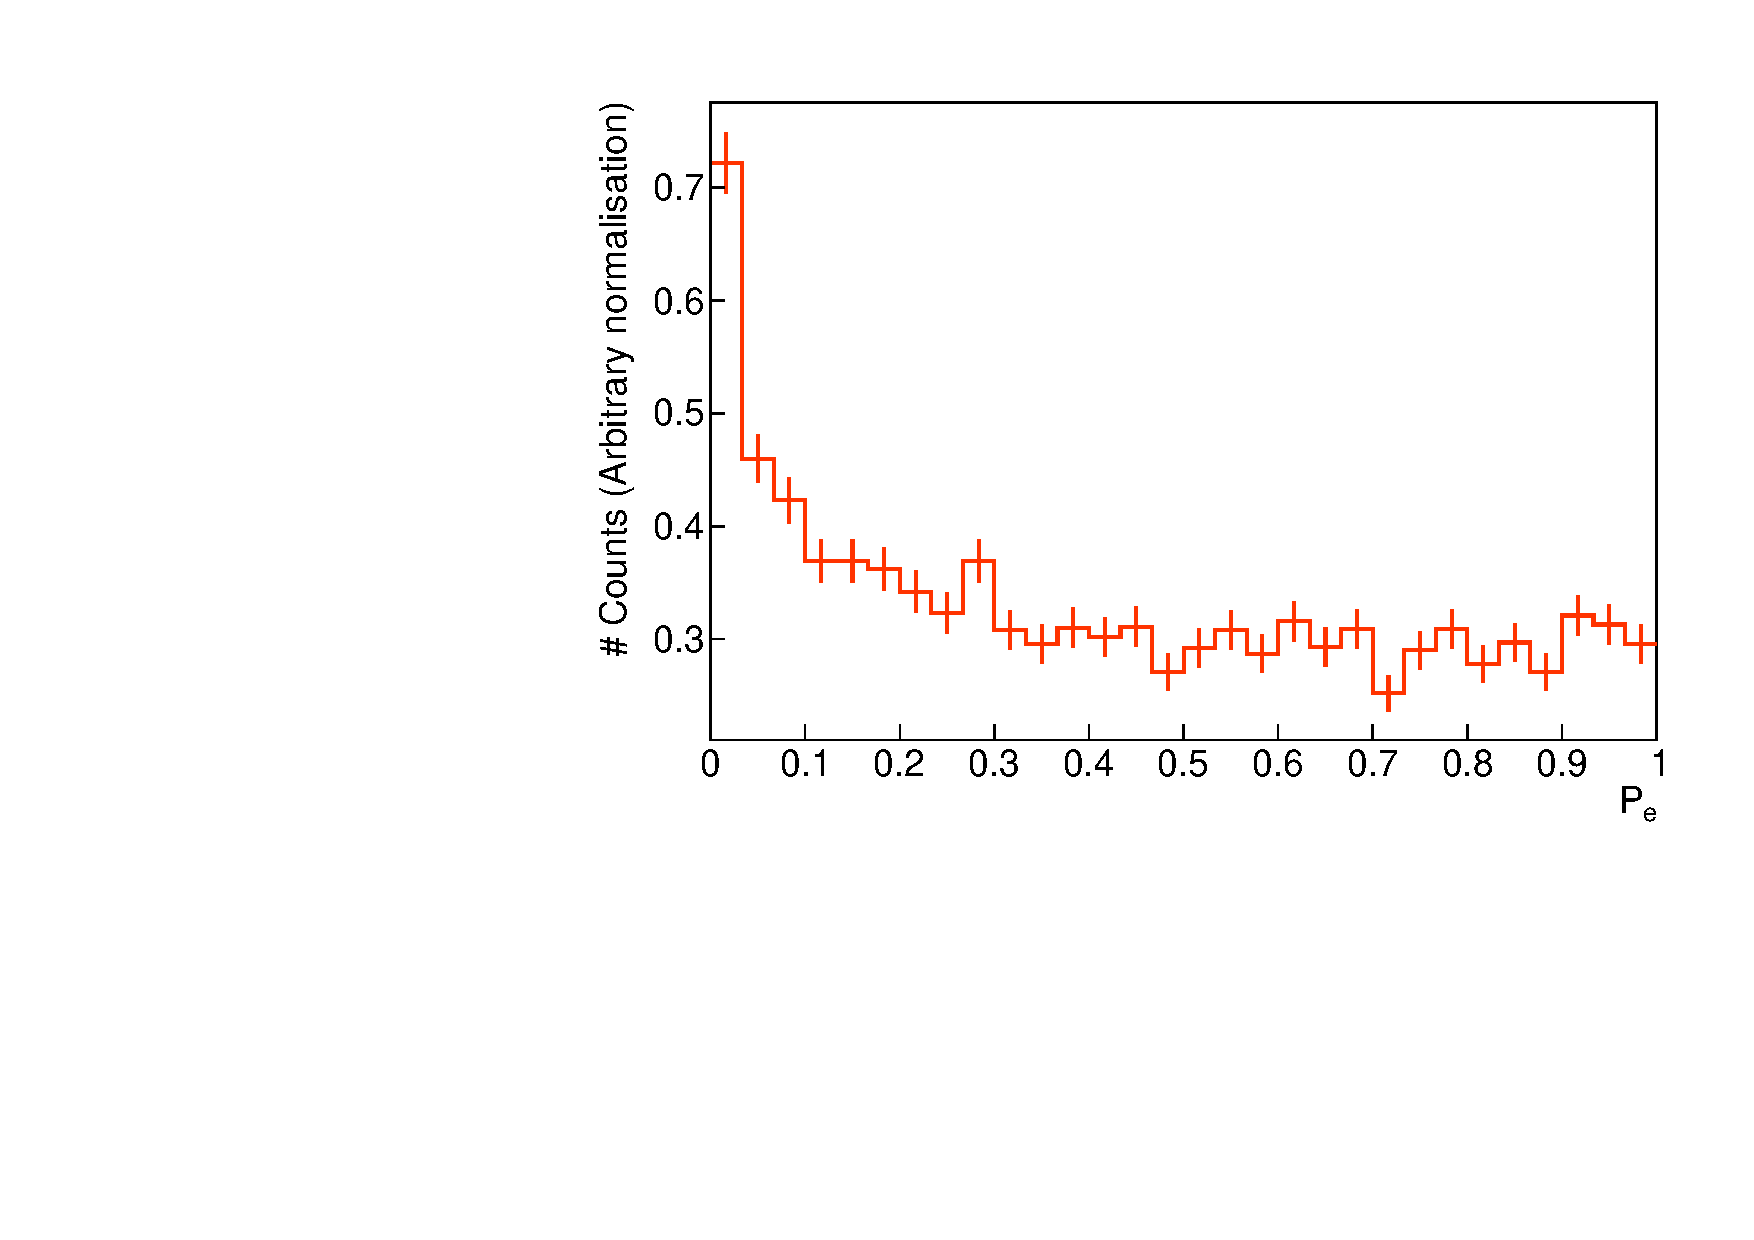
\includegraphics[width=13cm]{timedifference/fig_timediff/208Tl_expo.pdf}
  \caption{Exponential probability distributions for \Tl\ (red) and $\zeronu$ (green) simulations, after first-order cut-offs applied.
    $\sigma_{t}=0.400$~ns, $\sigma_{l}=0.0278$~ns.
    \label{fig:Pexp_Tl}}
\end{figure}
The


\section{Event selection}

\subsection{Selection on particle detection times}

After an event is tagged as a $2e$ topology, we consider the two arrival times of the electrons inside the calorimeter.
The time $t_{1}$ defines the arrival time of the highest energy particle, and the time $t_{2}$ designates the other.
The time difference between the two arrival times is then defined as
\begin{equation}
\Delta t~=~t^{\text{meas}}_{1}-t^{\text{meas}}_{2}\,.
\end{equation}
The time $t_{i}^{\text{meas}}$ it takes for a particle to reach the calorimeter depends on how long it took for it to exit the source foils after emission, as well as how long it took for it to travel through the wire chamber.
In order to remove from $\Delta t$ the dependency on travel time in the tracker, we define the corrected time difference as
\begin{equation}
\Delta t^{\text{corr}} = (t^{\text{meas}}_{1} - t^{\text{exp}}_{1}) - (t^{\text{meas}}_{2} - t^{\text{exp}}_{2})\,,
\end{equation}
where $t^{\text{exp}}_{i}$ is the expected arrival time, calculated with the particle energy and track length.

The two distributions $\Delta t$ and $\Delta t^{\text{corr}}$ are presented in Fig.~\ref{fig:delta_t}, for $\zeronu$ and \Tl\ simulations inside the source foils.
\begin{figure}[!h]
\centering
\begin{subfigure}[t]{1.\textwidth}
  \centering
  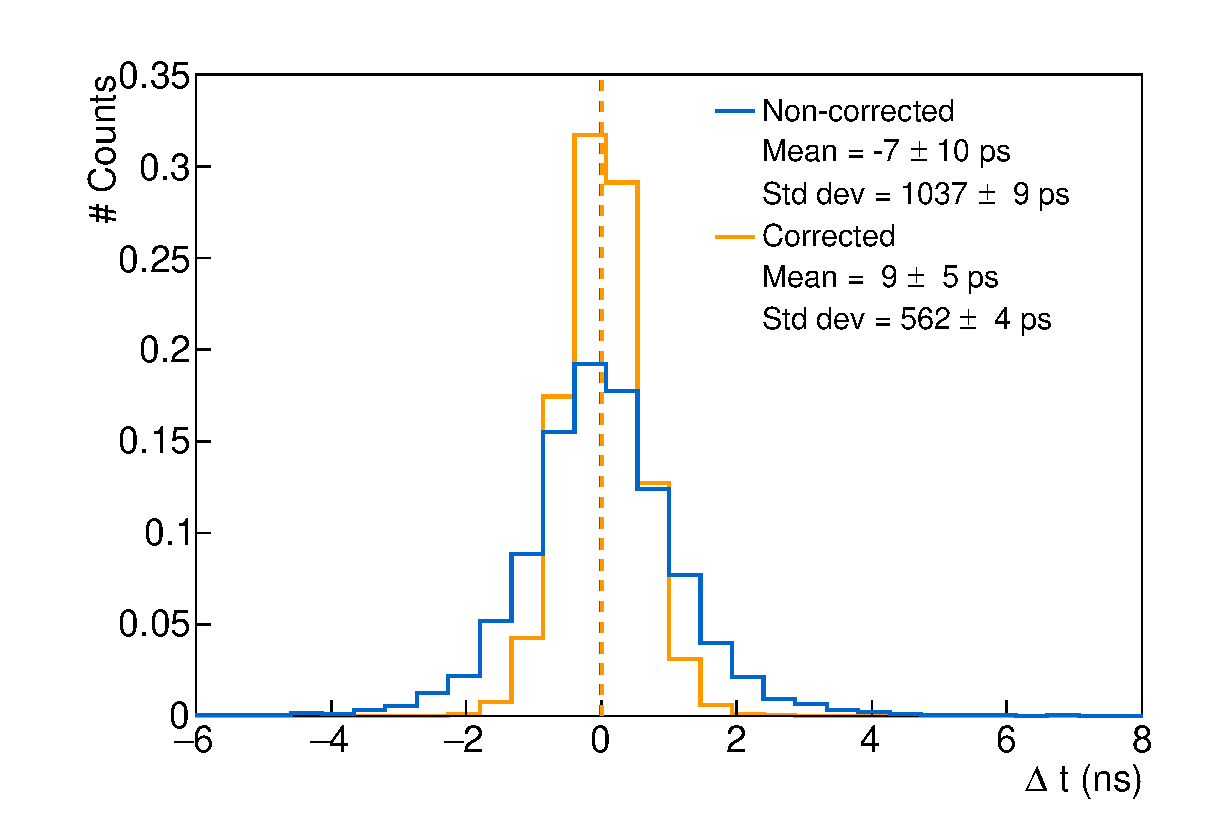
\includegraphics[width=0.82\textwidth]{timedifference/fig_timediff/0nubb_delta_t.eps}
  \captionsetup{justification=justified}
  \caption{$\zeronu$ simulations.
    \label{subfig:0nubb_delta_t}}
\end{subfigure}
\hfill
\begin{subfigure}[t]{1.\textwidth}
  \centering
  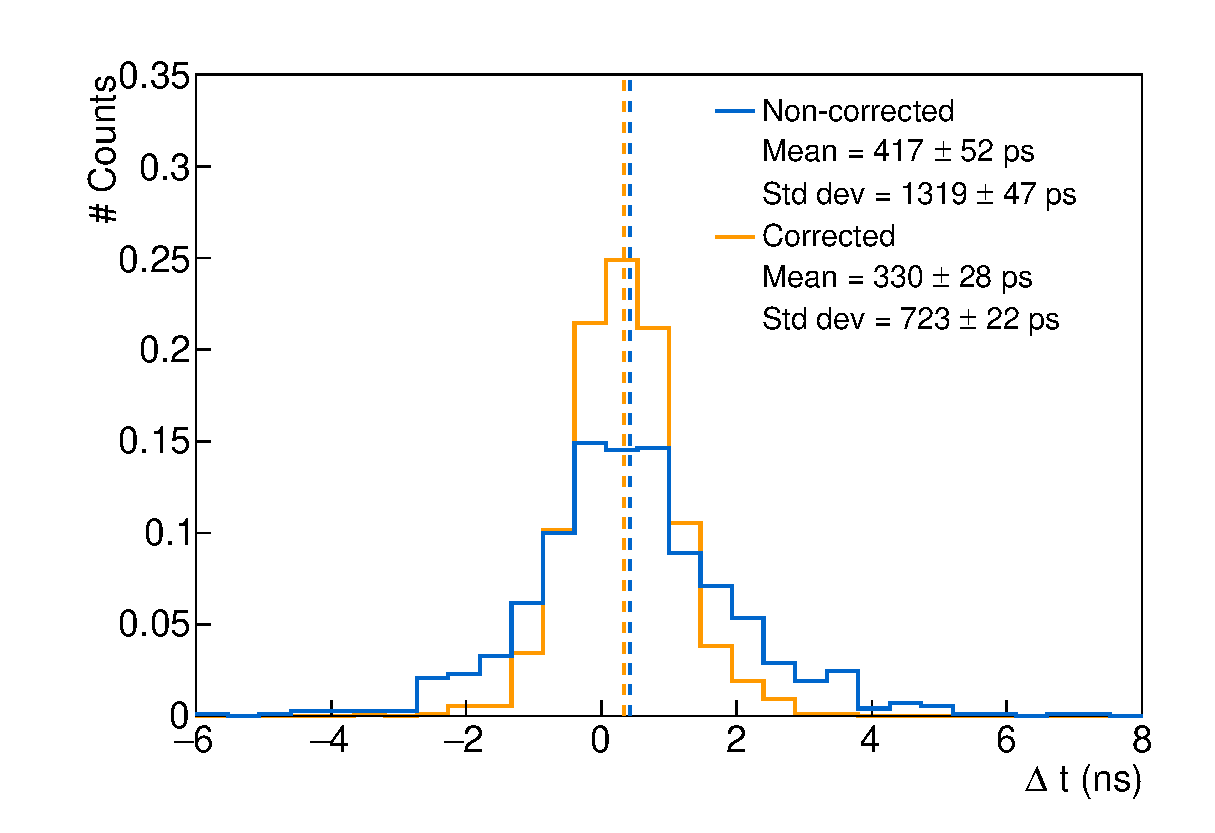
\includegraphics[width=0.82\textwidth]{timedifference/fig_timediff/208Tl_delta_t.eps}
  \captionsetup{justification=justified}
  \caption{\Tl\ simulations.
    \label{subfig:208Tl_delta_t}}
\end{subfigure}
\caption{Corrected (orange) and non-corrected (blue) arrival time difference between the two electrons.
  (a) $\zeronu$ simulations inside the source foils.
  (b) \Tl\ simulations inside the source foils.
  The first-order selections have been applied.
  The two distributions are normalised.
  $\sigma_{t}=0.400$~ns and $\sigma_{l}=0.0278$~ns.
  \label{fig:delta_t}}
\end{figure}
For $\zeronu$ simulations, the $\Delta t$ distribution is centred around zero, as expected.
Indeed, the two electrons of highest and lowest energy are not expected to be delayed.
Then, the correction on time difference only lowers the standard deviation of the distribution.
However, the mean of the $\Delta t$ distribution for \Tl\ events is slightly shifted towards negative values to $-0.218~\pm~0.013$~ns.
This is an indication of the existence of $\beta$+IC events, delaying the arrival time $t^{\text{meas}}_{1}$ of the particle of highest energy.

A simple way of rejecting \Tl\ delayed events consists in considering the sign $\Delta t^{\text{corr}}$.
We want to select $2e$ topology arising from $\beta$+IC delayed decays.
These events are more likely to present $t_{1}~<~t_{2}$, and therefore $\Delta t~<~0$.

\begin{itemize}
\item cut Pint/Pexp
\item Montrer un biplot Pint/Pexp pour les evts Tl208 en représentant la coupure.
\item Optimisation of event selection: cut on delta t
\item 208Tl cut efficiency
\item cut efficiencies on 0nubb and other backgrounds
\item Donner le nb d'ev rejeté sur le nb d'ev total, puis sur le nb d'ev retardés
\item relier coupure sur proba avec coupure sur delta t (<0,>0)
\end{itemize}

\section{Impact of \Tl\ rejection on the experiment's sensitivity}
Reprendre l'analyse de sensibilité faite avec Axel en rajoutant les cuts Pint/Pexp et delta t pour le final detector

\subsection{Influence of the calorimeter time resolution}

\begin{figure}
  \centering
  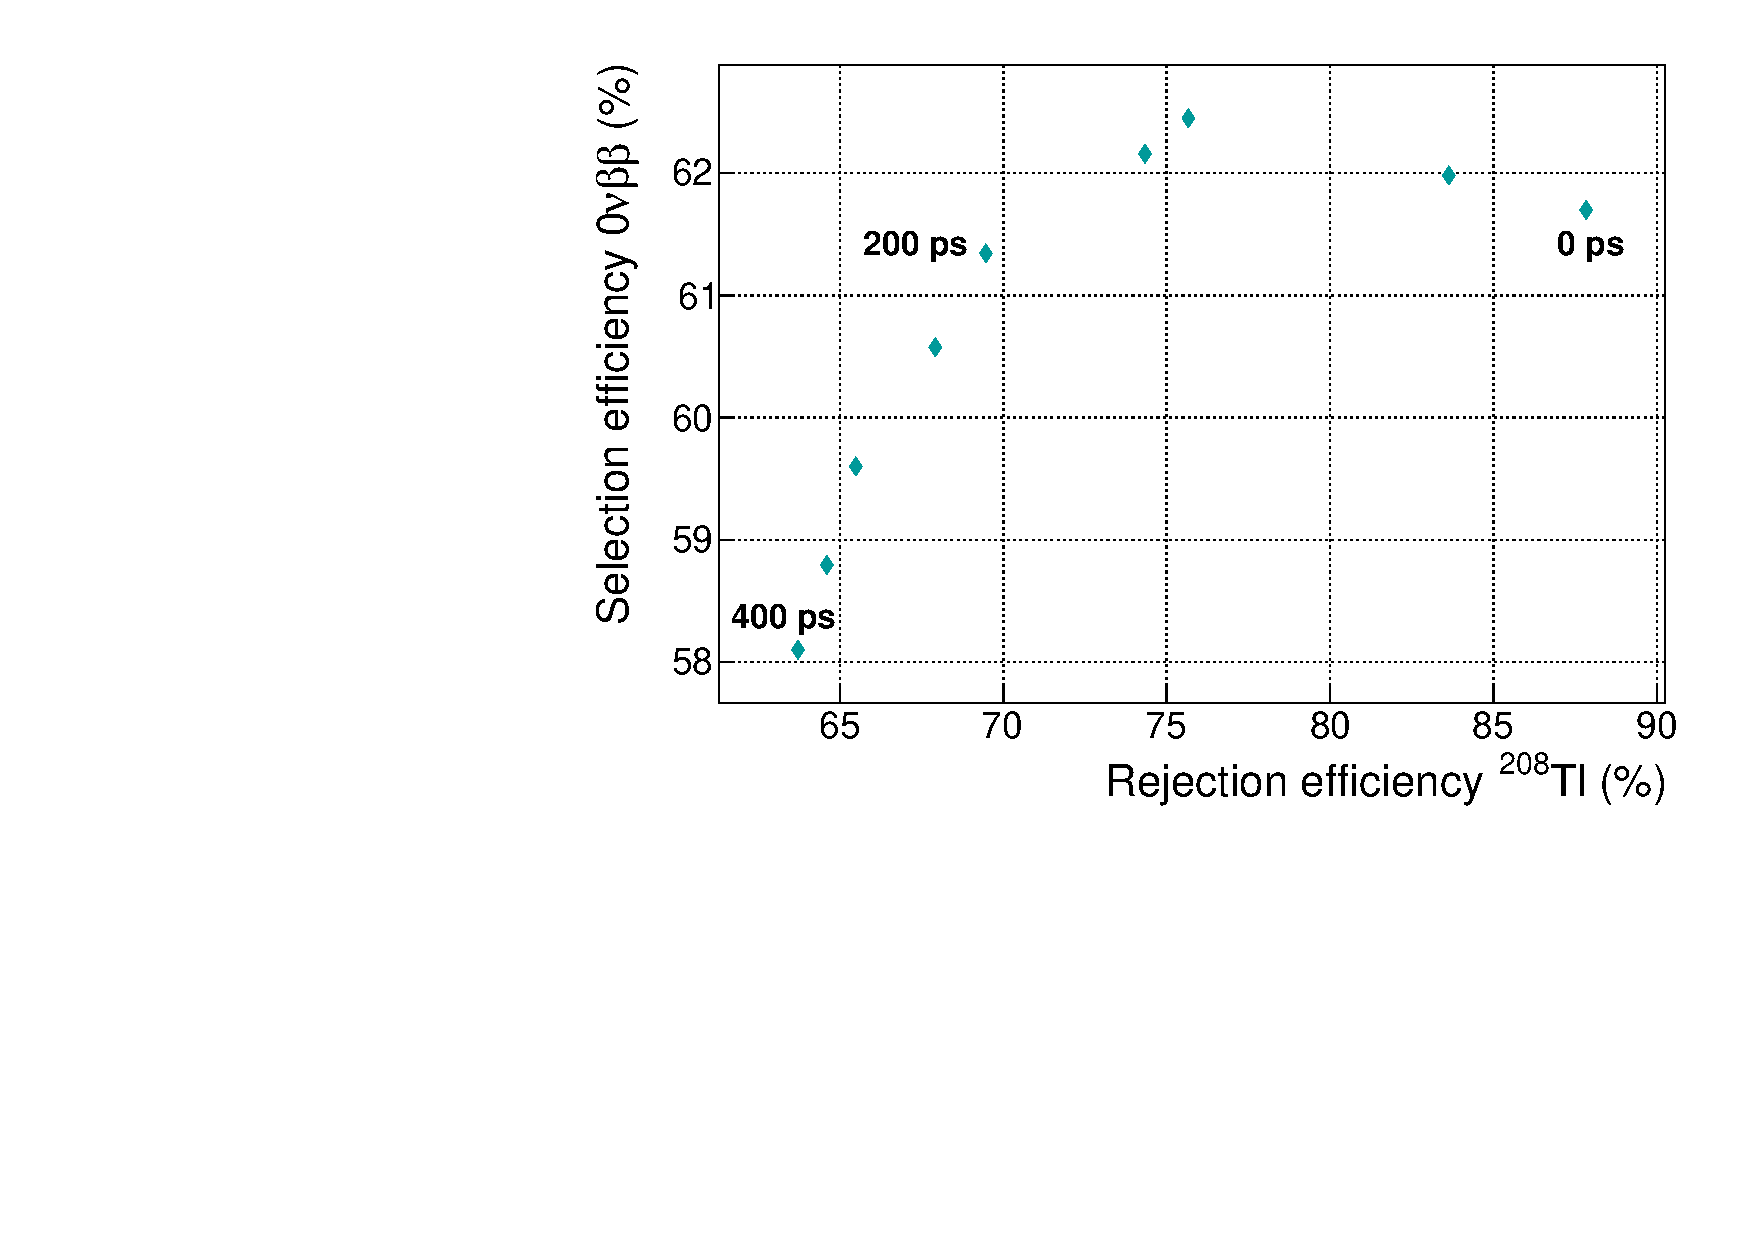
\includegraphics[width=13cm]{timedifference/fig_timediff/efficiency_proba.pdf}
  \caption{$\zeronu$ selection efficiency as a function of \Tl\ rejection efficiency.
    Each data point corresponds to a given value of $\sigma_{t}$, decrementing in $50$~ps steps.
    First order selections applied on $\zeronu$ and \Tl\ simulations.
    $\sigma_{l}=0.0278$~ns.
    \label{fig:eff_proba_sigma}}
\end{figure}

\begin{figure}
  \centering
  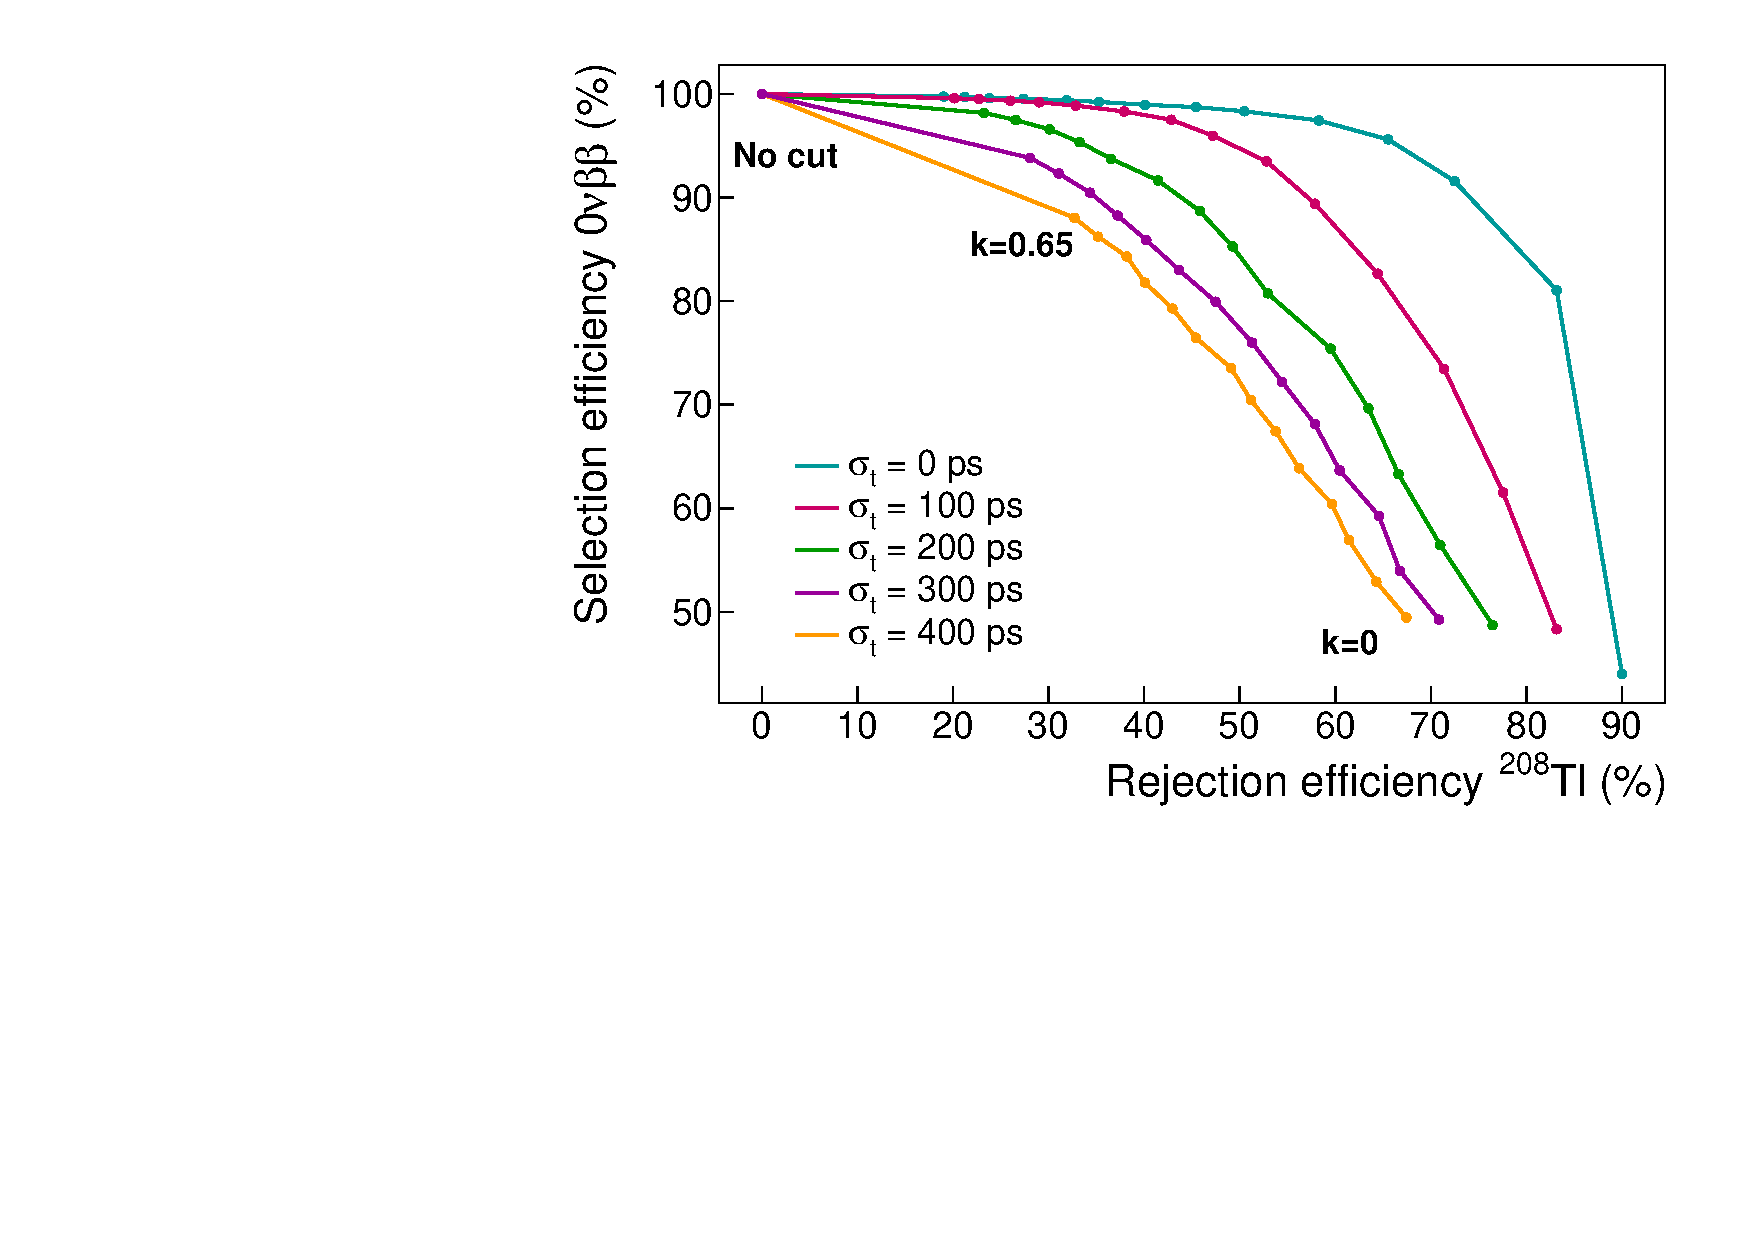
\includegraphics[width=13cm]{timedifference/fig_timediff/compare_sigma_cut_delta_t.pdf}
  \caption{$\zeronu$ selection efficiency as a function of \Tl\ rejection efficiency.
    Each data point corresponds to a given value of $\sigma_{t}$, decrementing in $50$~ps steps.
    First order selections applied on $\zeronu$ and \Tl\ simulations.
    $\sigma_{l}=0.0278$~ns.
    \label{fig:eff_cut_delta_t_sigma}}
\end{figure}

\begin{figure}
  \centering
  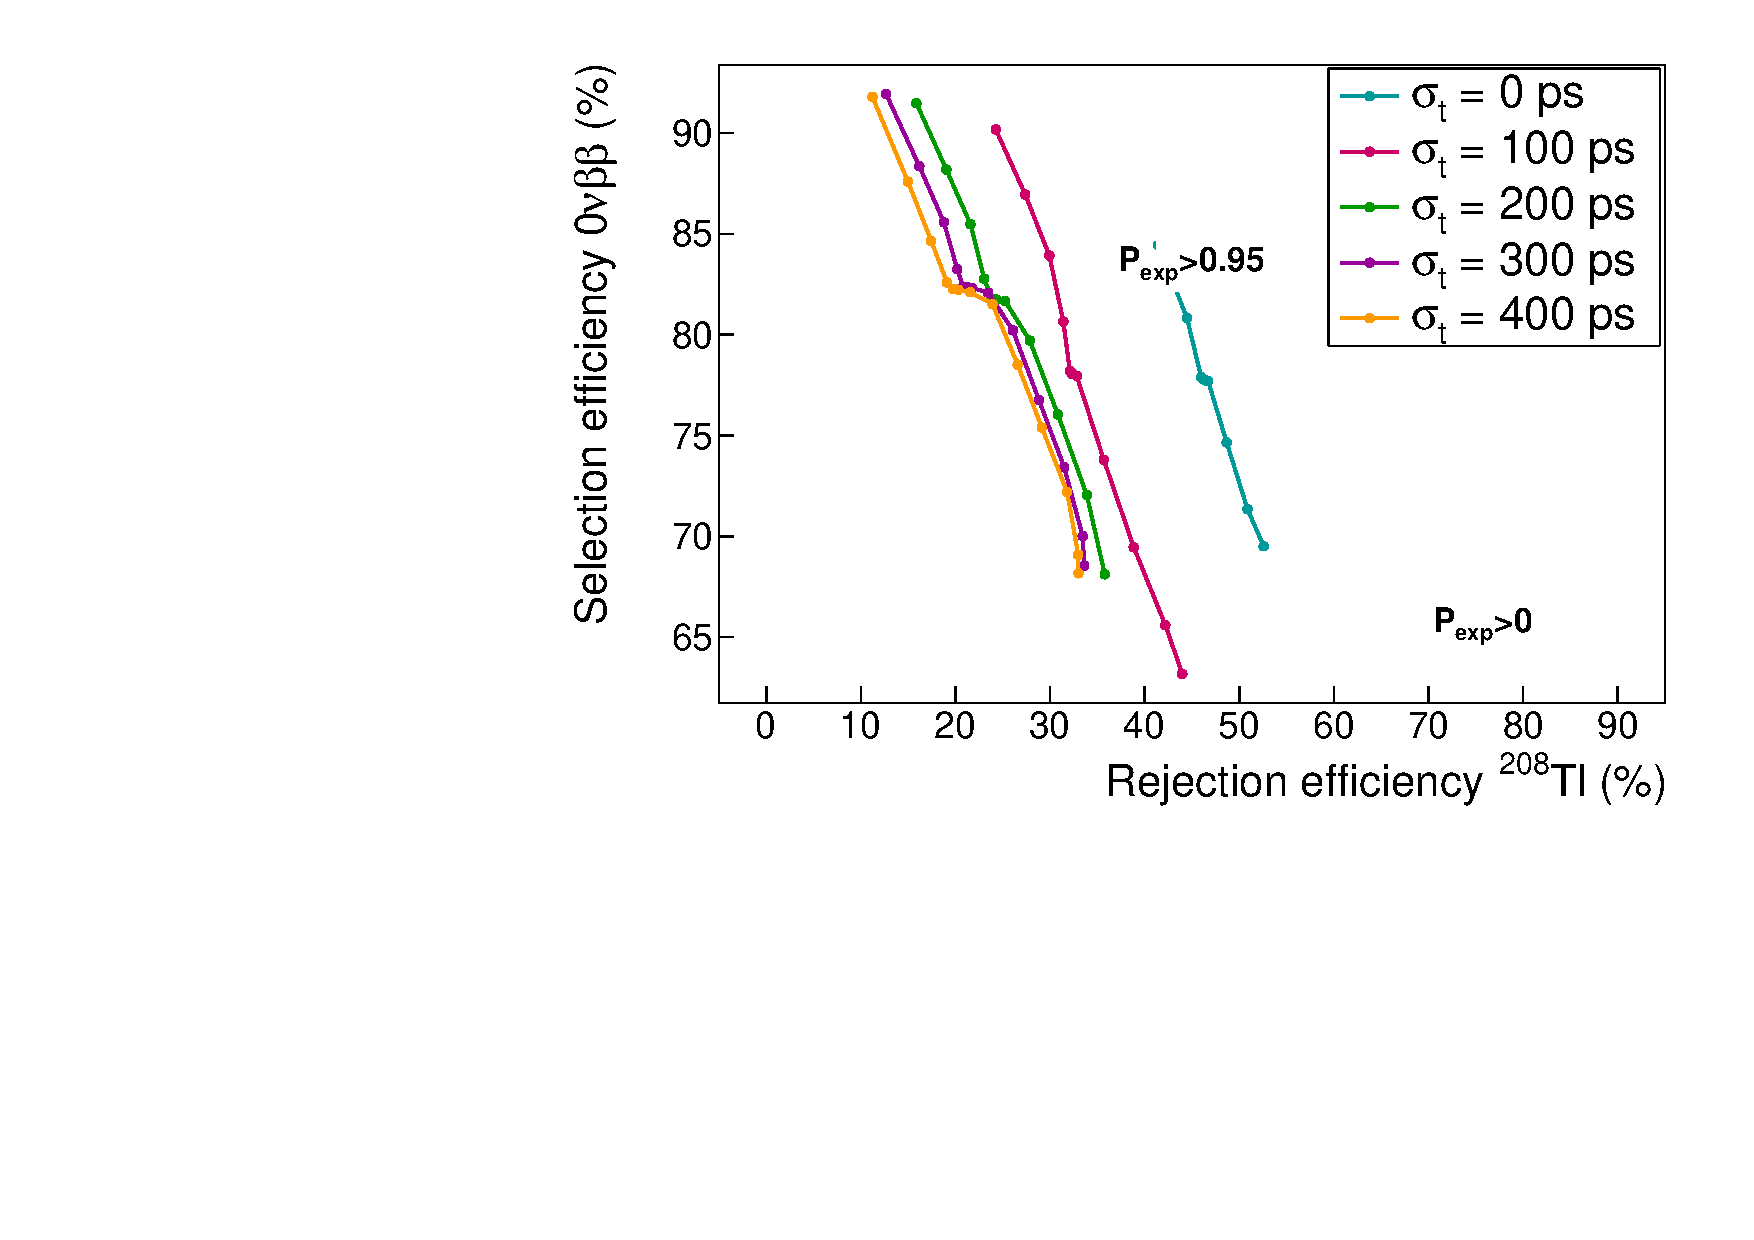
\includegraphics[width=13cm]{timedifference/fig_timediff/compare_sigma_cut_proba.pdf}
  \caption{$\zeronu$ selection efficiency as a function of \Tl\ rejection efficiency.
    Each data point corresponds to a given value of $\sigma_{t}$, decrementing in $50$~ps steps.
    First order selections applied on $\zeronu$ and \Tl\ simulations.
    $\sigma_{l}=0.0278$~ns.
    \label{fig:eff_cut_proba_sigma}}
\end{figure}

\begin{itemize}
\item Se servir des résultats de $\sigma_{t}$ trouvés au chap.~\ref{chap:Cobalt_study}
\item Mais dire que ces sigmas peuvent être améliorés
\item donc présenter l'évolution des résultats (efficacité de réjection et sensibilité) sur la réjection en fonction de la valeur de sigma t, à faire varier dans un certain range.
\item Tu pourrais avec une figure à 2D où tu montres l'efficacité relative 0nu (égale à 100\% avant cette coupure temporelle) en fonction de la réjection du Tl208 -> cela donne une courbe que tu parcoures et tu cherches à optimiser ton point de fonctionnement.
\end{itemize}


\section{Conclusions}

\begin{itemize}
\item On peut éventuellement mettre une source de 232U dans le détecteur (un des parents de 208Tl) pour tester la réjection.
\item ajout sélection énergie
\end{itemize}


\begin{figure}
  \centering
  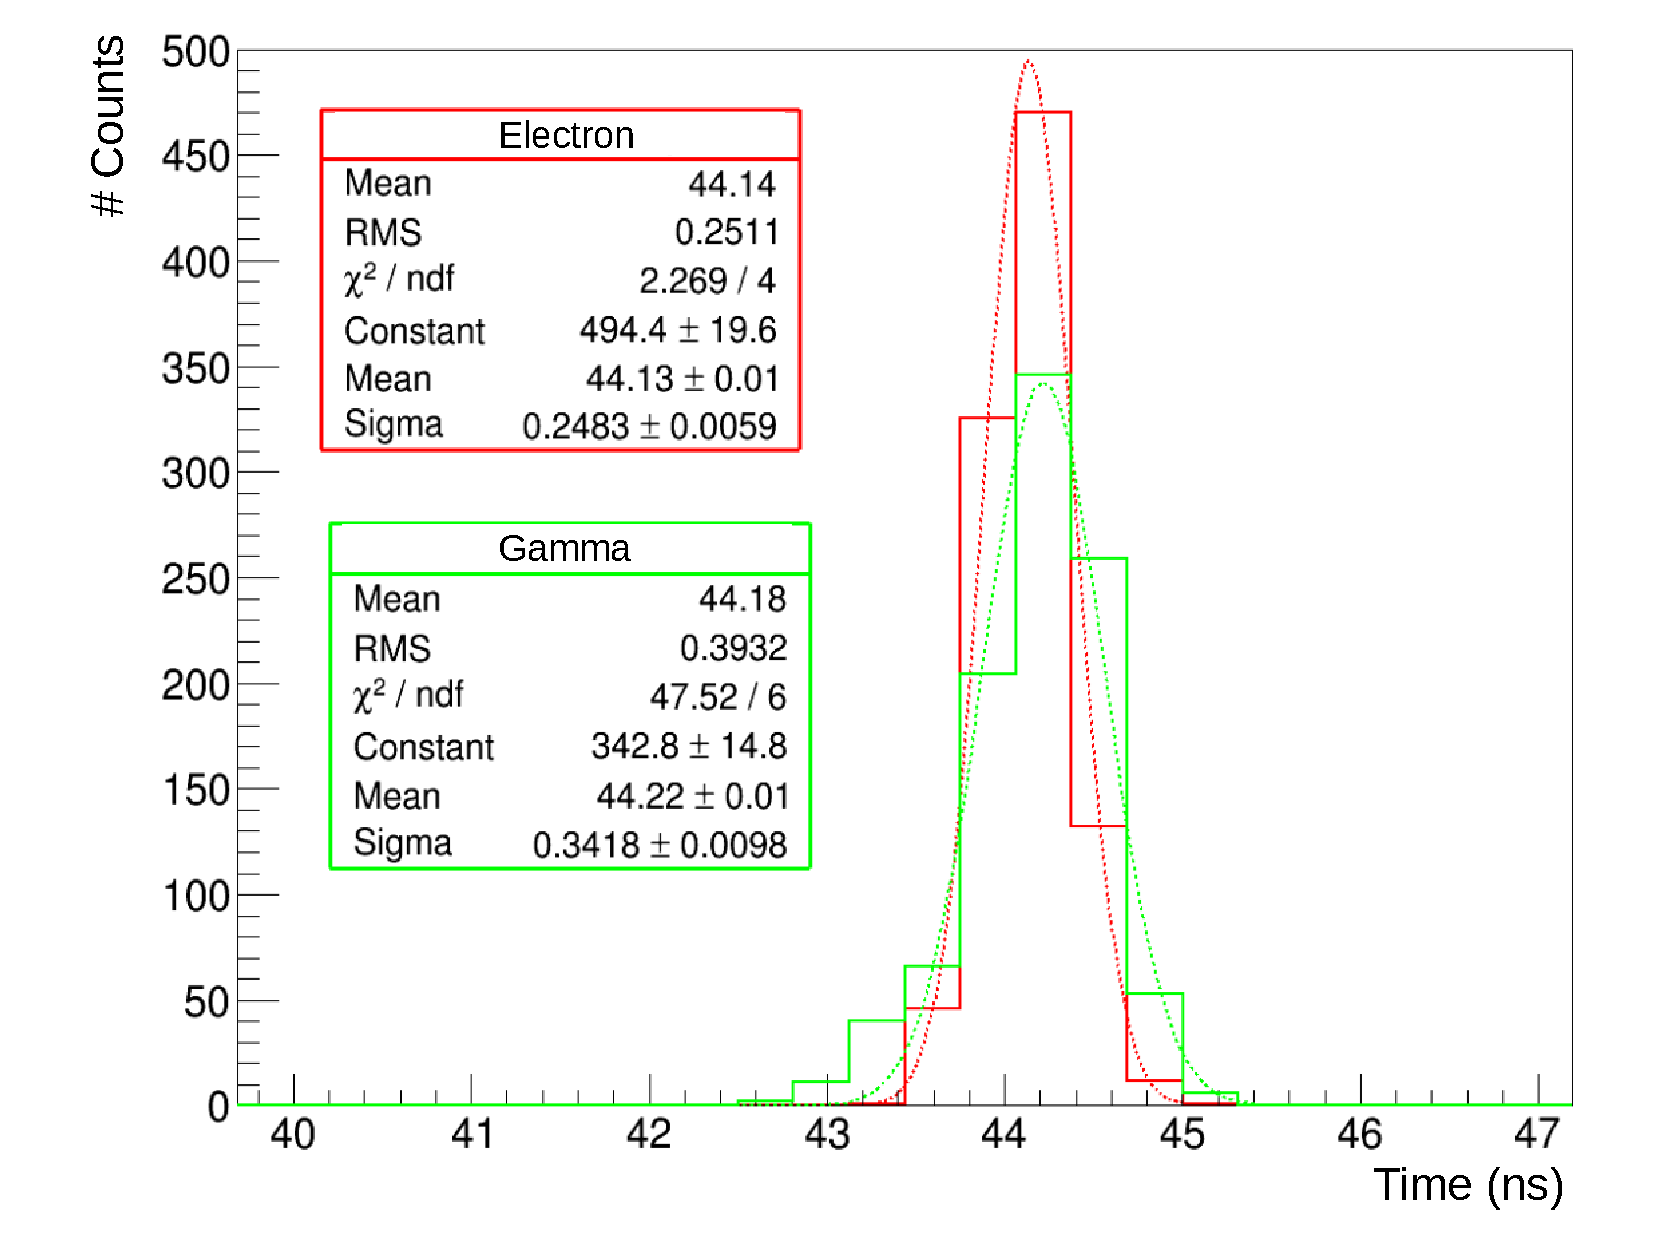
\includegraphics[width=13cm]{timedifference/fig_timediff/Arnaud_RMS_PM.pdf}
  \caption{Time distribution of the trigger time of an optical module in the case of electrons (red) and gamma radiation (green) depositing an energy of $1$~MeV in the scintillator.
    The trigger threshold is set at $45$ mV and corresponds to an energy of $0.150$~MeV.
    Adapted from~\cite{HuberThesis}.
  \label{fig:Arnaud_RMS_PM}}
\end{figure}
